% =====================================================================
%  Chapitre 2 -- Le RNN : architecture et propagation
%  Partie a : deroulement, cellule, etat cache, BPTT
% =====================================================================
\section{Chapitre 2 --- Architecture RNN}

\chapterslide{Chapitre 2}{Le RNN : architecture et propagation}%
{6 h --- déroulement temporel, cellule, BPTT, gradients}%
{\textbf{Objectifs.} Écrire les équations d'une cellule récurrente ; comprendre le
déroulement temporel et la réutilisation des poids ; dérouler la rétropropagation
à travers le temps ; expliquer le gradient qui s'évanouit par le calcul.}

\begin{frame}{L'idée en une phrase}
\begin{kbox}[Une cellule, un état, beaucoup de pas]
Le réseau ne change pas d'un pas de temps à l'autre : c'est la \textbf{même
cellule}, avec les \textbf{mêmes poids}, appliquée successivement à chaque
élément de la séquence.

\medskip
Entre deux pas, elle transmet un \textbf{état caché} $h_t$ --- sa mémoire de
ce qu'elle a déjà lu.
\end{kbox}
\vspace{2mm}
\begin{wbox}[Ce que cela implique]
Le nombre de paramètres ne dépend pas de la longueur de la séquence :
une phrase de 5 mots et une de 500 passent par le même réseau.
\end{wbox}
\end{frame}

\begin{frame}{Le déroulement temporel (unrolling)}
\begin{center}
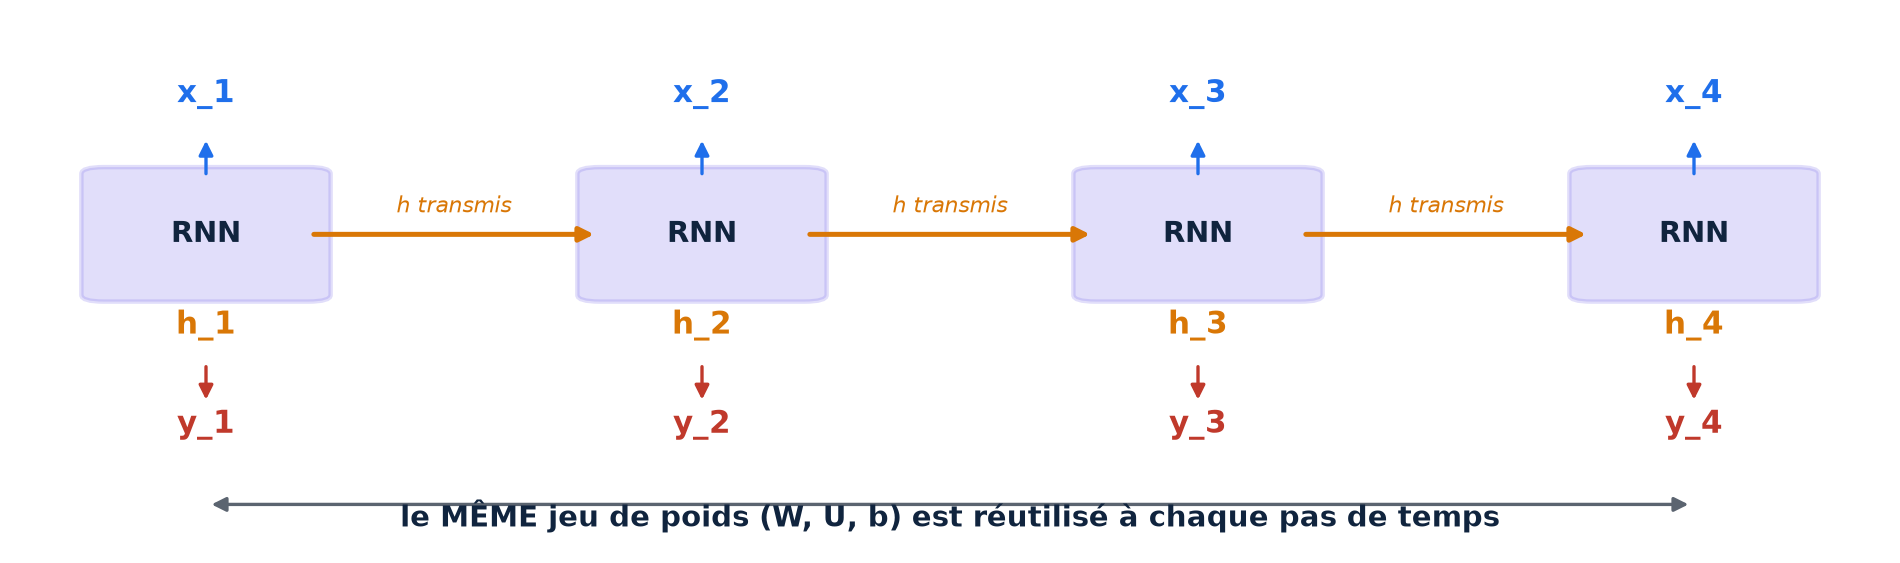
\includegraphics[width=0.95\textwidth]{s01_deroulement.png}
\end{center}
\vspace{1mm}
\begin{itemize}
  \item À gauche : une boucle. À droite : la même chose, déroulée dans le temps.
  \item Les boîtes sont \textbf{la même} cellule : mêmes poids, même biais.
  \item Le trait orange est l'état caché transmis.
\end{itemize}
\end{frame}

\begin{frame}[fragile]{La cellule, en une équation et cinq lignes}
\begin{columns}[t]
\begin{column}{0.48\textwidth}
\begin{codebox}[PyTorch, à la main]
\begin{lstlisting}
def cellule(x_t, h_pre):
    return torch.tanh(
        Wx @ x_t + Wh @ h_pre + b)

h = torch.zeros(H)
for x_t in sequence:
    h = cellule(x_t, h)
\end{lstlisting}
\end{codebox}
\end{column}
\begin{column}{0.48\textwidth}
\begin{center}
$h_t = \tanh(W_x\, x_t + W_h\, h_{t-1} + b)$
\end{center}
\vspace{1mm}
\begin{itemize}
  \item $W_x$ : comment l'entrée du pas pénètre.
  \item $W_h$ : comment la mémoire se maintient.
  \item $\tanh$ : garde $h_t$ dans $[-1, 1]$.
\end{itemize}
\end{column}
\end{columns}
\end{frame}

\begin{frame}{L'état caché en action}
\begin{center}
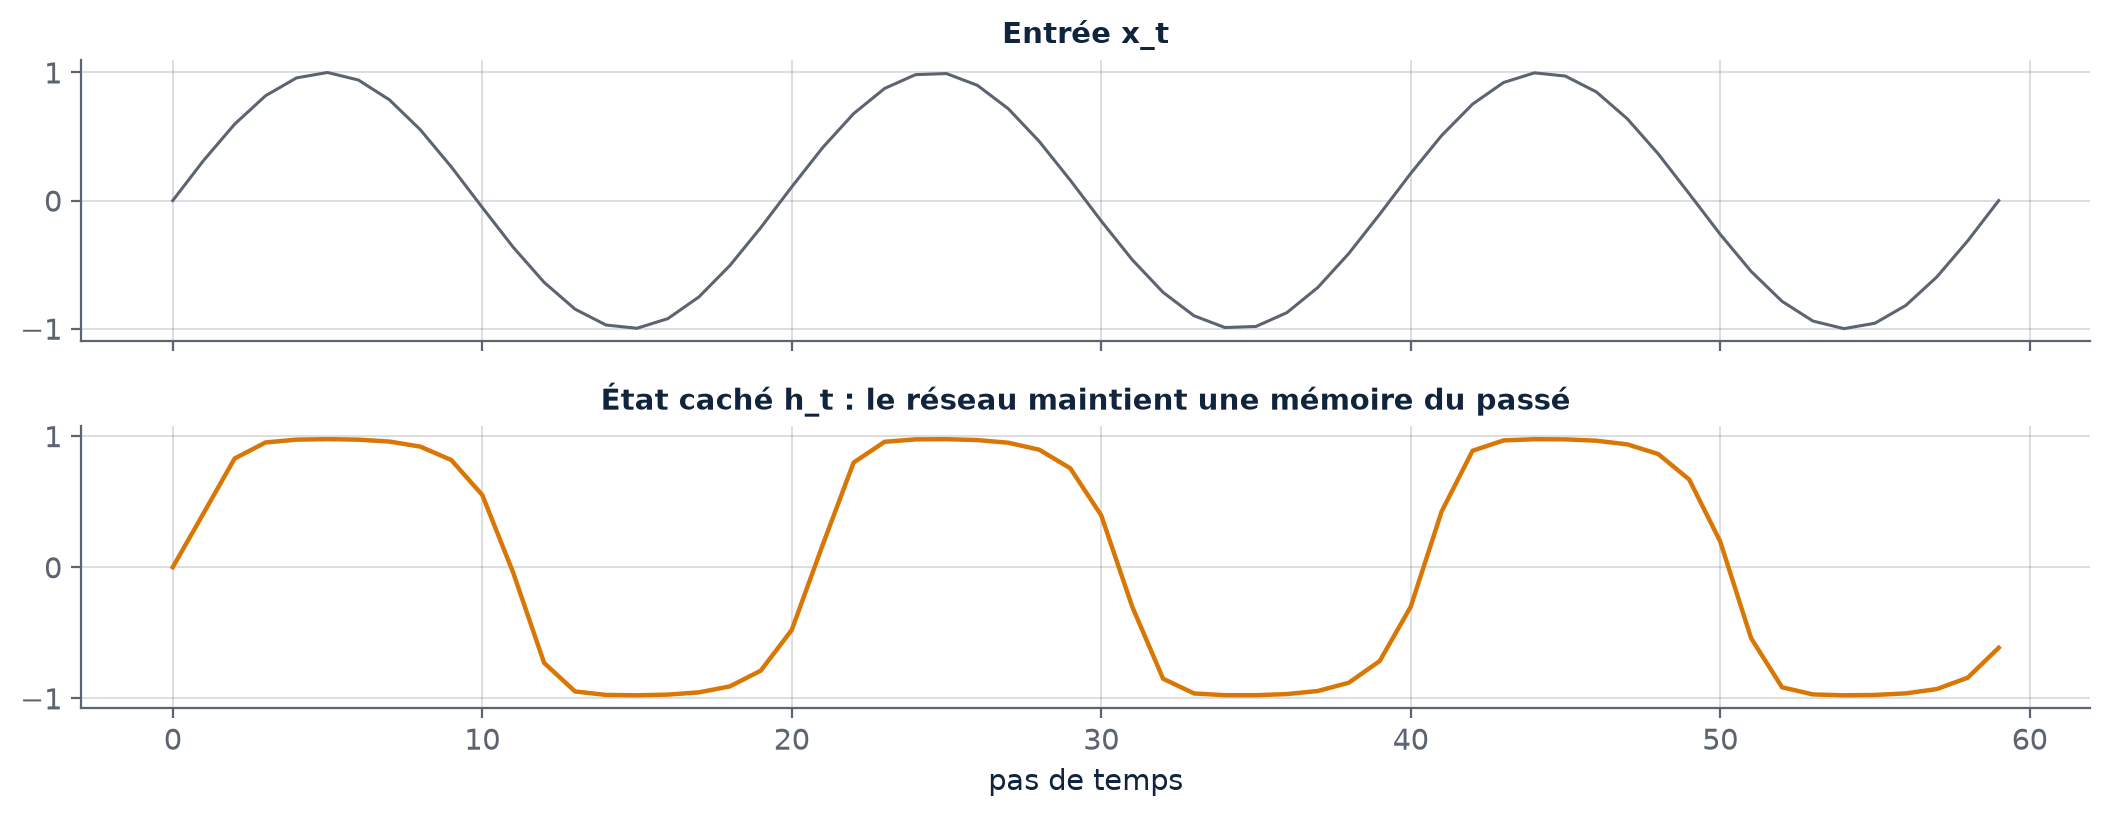
\includegraphics[width=0.88\textwidth]{s03_etat_cache.png}
\end{center}
\vspace{1mm}
\begin{kbox}[Une mémoire vivante]
L'état $h_t$ suit l'entrée, la lisse, la retarde : il encode un \textbf{résumé
mobile} de tout ce qui a été vu jusqu'ici.
\end{kbox}
\end{frame}

\begin{frame}{Combien de paramètres ?}
\begin{columns}[t]
\begin{column}{0.96\textwidth}
\begin{itemize}
  \item Une couche RNN : $E \times H + H \times H + H$ paramètres
  (entrée, récurrence, biais).
  \item \textbf{Aucun} terme ne dépend de la longueur $T$.
  \item La même matrice $W_h$ s'applique $T$ fois : c'est le partage de poids
  du CNN, version temporelle.
\end{itemize}
\begin{solbox}[Repère du cours]
$E = 300$, $H = 128$ : $300 \times 128 + 128 \times 128 + 128
= 54\,784$ paramètres.
\end{solbox}
\end{column}
\end{columns}
% [fix] figure sortie
\end{frame}

\begin{frame}{Combien de paramètres ? --- la figure}\begin{center}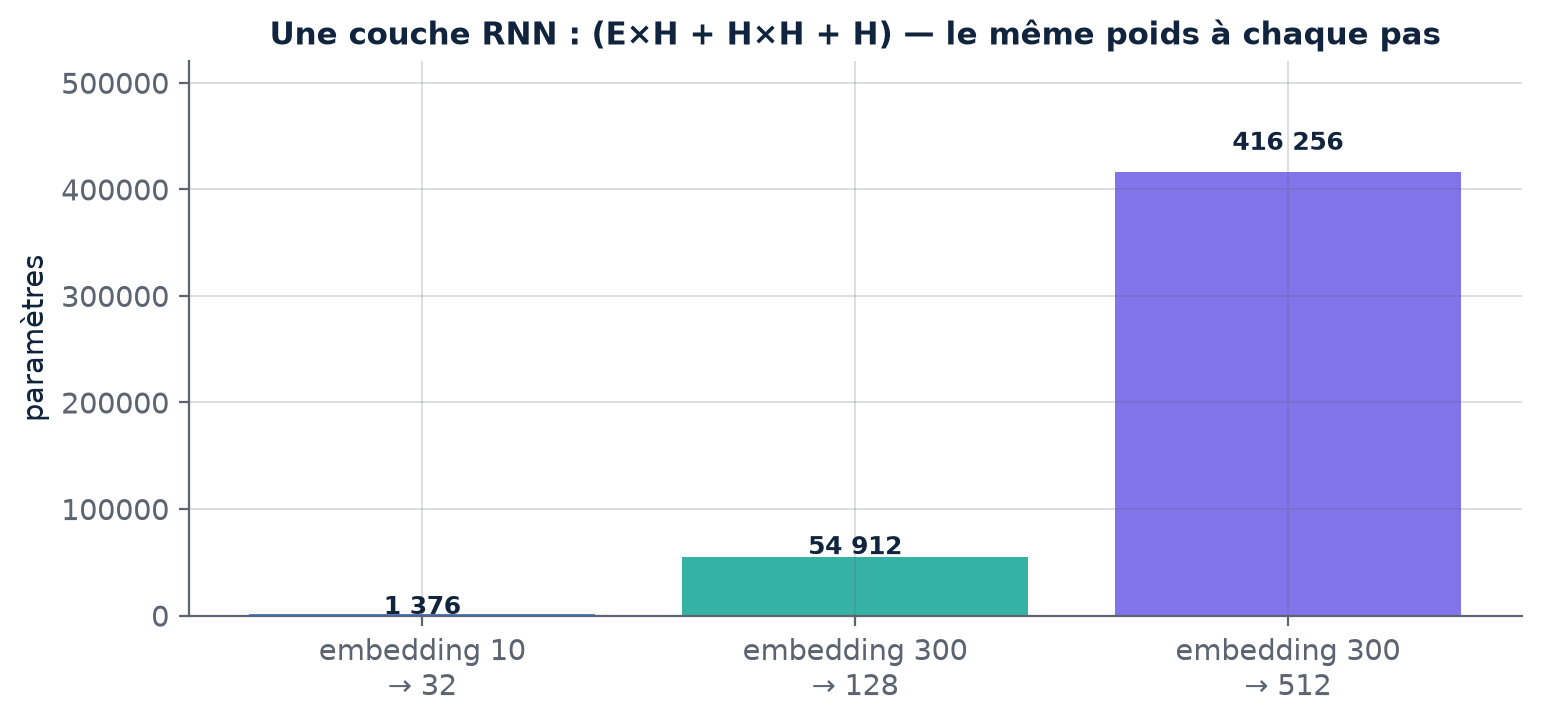
\includegraphics[width=.92\textwidth]{s09_parametres.png}\end{center}\end{frame}

\begin{frame}{Entraîner : la rétropropagation à travers le temps}
\begin{center}
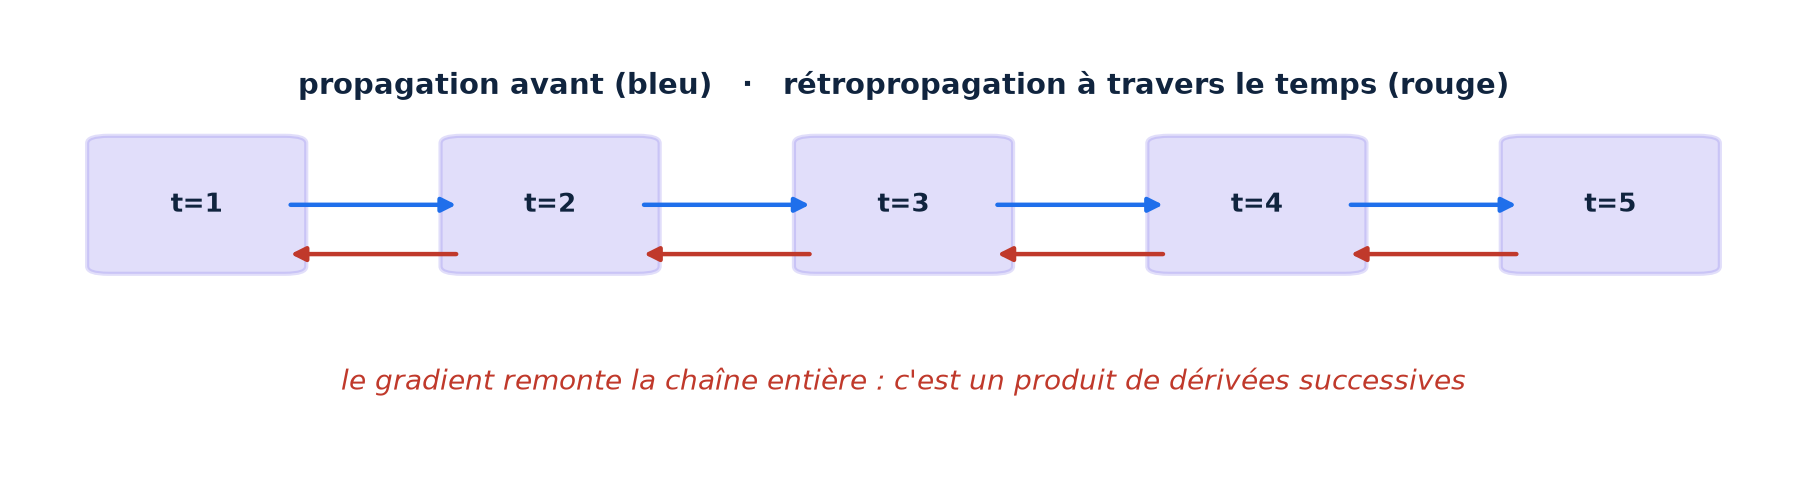
\includegraphics[width=0.94\textwidth]{s04_bptt.png}
\end{center}
\vspace{1mm}
\begin{itemize}
  \item On déroule, on calcule la perte, puis le gradient \textbf{remonte}
  la chaîne dans le sens inverse du temps.
  \item Le gradient qui atteint le pas 1 a traversé \textbf{tous} les pas
  intermédiaires.
\end{itemize}
\end{frame}

\begin{frame}{Le problème, formulé proprement}
\begin{columns}[t]
\begin{column}{0.52\textwidth}
\begin{kbox}[Le gradient le long du temps]
Pour remonter $T$ pas, le gradient contient un produit :
\[
\frac{\partial h_t}{\partial h_0}
\approx \prod_{k=1}^{t} W_h^{\,\top} \operatorname{diag}(\tanh')
\]
\end{kbox}
\begin{itemize}
  \item Si la norme de chaque facteur vaut $< 1$ : le produit tend vers 0
  --- gradient \textbf{évanouissant}.
  \item Si elle vaut $> 1$ : le produit explose.
\end{itemize}
\end{column}
\begin{column}{0.44\textwidth}
\begin{wbox}[Ni l'un ni l'autre n'est bon]
\begin{itemize}
  \item Évanouissant : le réseau \textbf{oublie} le début de la séquence.
  \item Explosant : les mises à jour détruisent les poids.
\end{itemize}
Le chapitre 3 règle le premier cas ; le clipping règle le second.
\end{wbox}
\end{column}
\end{columns}
\end{frame}

\begin{frame}{La preuve par le calcul}
\begin{columns}[t]
\begin{column}{0.96\textwidth}
\begin{itemize}
  \item Chaque courbe est un \textbf{calcul exact} : $r^{t}$ pour un rayon
  spectral $r$ de la matrice de récurrence.
  \item $r = 0{,}55$ : après 20 pas, il reste $0{,}55^{20} \approx 6 \times
  10^{-6}$ du gradient.
  \item $r = 1{,}35$ : après 20 pas, $\approx 406$ — et cela continue.
\end{itemize}
\begin{solbox}[Repères du cours]
$r = 0{,}55$ : $r^{20} = 6{,}4 \cdot 10^{-6}$ ;\quad
$r = 1{,}35$ : $r^{20} = 405{,}9$.
\end{solbox}
\end{column}
\end{columns}
% [fix] figure sortie
\end{frame}

\begin{frame}{La preuve par le calcul --- la figure}\begin{center}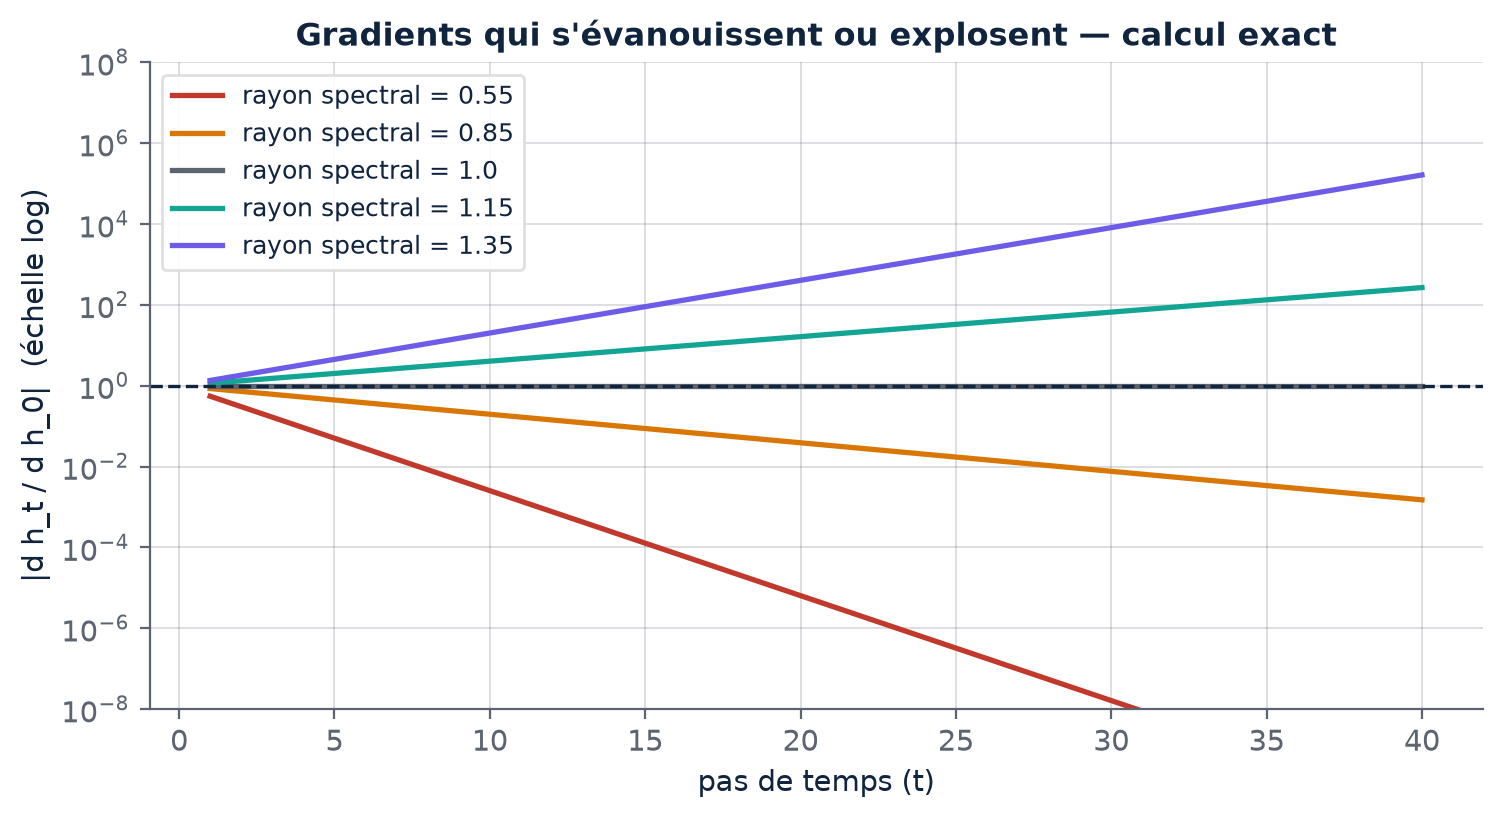
\includegraphics[width=.92\textwidth]{s05_gradients.png}\end{center}\end{frame}

\begin{frame}{Le clipping : traiter l'explosion}
\begin{center}
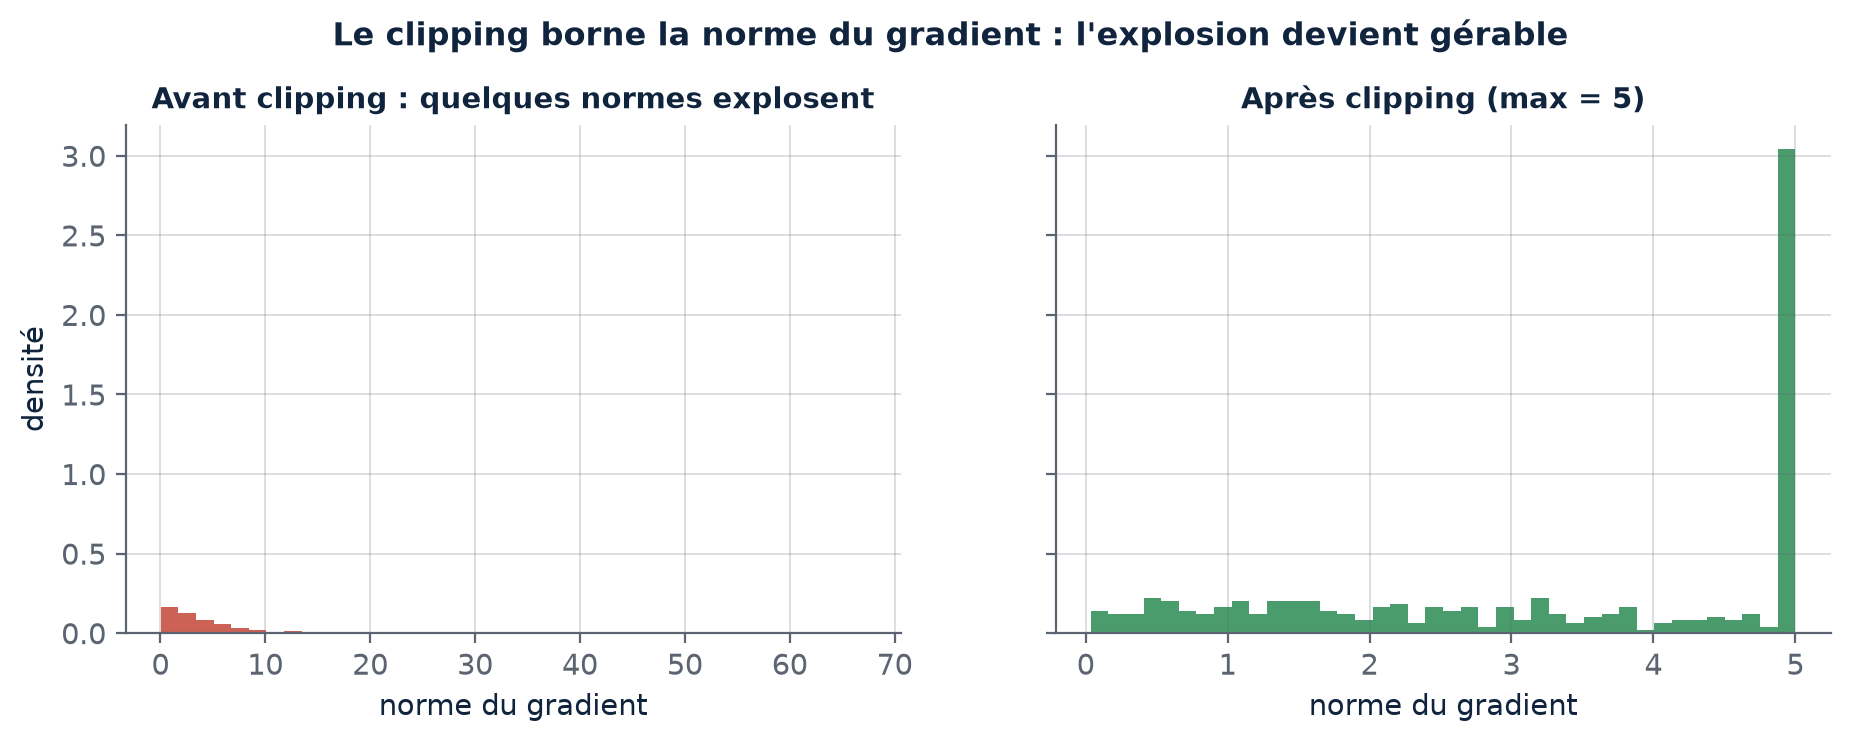
\includegraphics[width=0.86\textwidth]{s06_clipping.png}
\end{center}
\vspace{1mm}
\begin{itemize}
  \item On mesure la \textbf{norme} du gradient ; si elle dépasse un seuil
  (typiquement 5), on la ramène à ce seuil.
  \item Une ligne de code, un geste réflexe : \py{torch.nn.utils.clip_grad_norm_}.
\end{itemize}
\end{frame}
